\documentclass[11pt]{article}
\usepackage[margin=1in]{geometry}
\usepackage{amsmath,amssymb}
\usepackage{graphicx}
\usepackage{booktabs}
\usepackage{xcolor}
\usepackage{caption}
\usepackage[hidelinks]{hyperref}
\usepackage{authblk}
\usepackage{natbib}
\graphicspath{{../figures/}}
\captionsetup{font=small,labelfont=bf}
\newcommand{\D}{D}
\title{\bfseries Growing the Chicago `L': A Slime-Mold Physics Model for \\
Demand-Weighted, Constraint-Aware Rapid-Transit Expansion}
\author{Prepared for Charlie}
\date{June 2026}

\begin{document}
\maketitle

\begin{abstract}
\noindent The plasmodial slime mold \emph{Physarum polycephalum} builds transport
networks that trade total length against robustness and transport efficiency in a
way that rivals human-engineered systems, most famously reproducing the Tokyo rail
network in the laboratory \citep{tero2010}. We adapt the Tero current-reinforcement
model of \emph{Physarum} into a constrained optimization engine that \emph{grows} a
candidate expansion of the Chicago Transit Authority `L' rail system. Demand is
modeled as a convex blend of residential population, activity-center draw, and
transit-desert severity; geography enters as a hard Lake Michigan no-build boundary
and a spatially varying construction-cost field (right-of-way reuse discounts,
downtown tunnelling premiums) that the flow physics reads as an effective tube
length. On a $678$-node candidate lattice we evolve the conductivity field to a
self-organized network and benchmark it against minimum-spanning-tree, Steiner-tree,
and hub-and-spoke baselines using the Tero cost--benefit metrics (total length $TL$,
mean inter-terminal distance $MD$, fault tolerance $FT$). The balanced slime-mold
network ($\gamma=1.3$) costs $1.74\times$ the MST length but cuts the mean trip
distance by $30\%$ (to $18.8$\,km from $26.9$\,km) and raises fault tolerance from
$0$ to $0.89$; results are stable across random seeds ($FT=0.88\pm0.02$). A single
adaptation exponent $\gamma$ sweeps the network continuously from a redundant mesh
to a minimal tree, tracing a Pareto front the planner can select along. We release
the full code, data, and figures.
\end{abstract}

\section{Introduction}
Expanding a heavy-rail transit system is a constrained network-design problem: a
planner must connect many demand centers to an existing backbone, cheaply, while
keeping trips short and the system resilient to disruption. These goals conflict,
and the underlying combinatorial problem (minimum-cost connection of a terminal set
through optional intermediate junctions) is the NP-hard Steiner tree problem
\citep{hwang1992}.

Biology offers a remarkable heuristic. \emph{Physarum polycephalum}, a single-celled
slime mold, forms a network of protoplasm-carrying tubes between food sources and
continuously remodels it: tubes carrying strong flow thicken, idle tubes wither.
\citet{nakagaki2000} showed the organism solves shortest-path mazes; \citet{tero2010}
placed food sources at the cities surrounding Tokyo and obtained a network whose cost,
efficiency, and fault tolerance matched the real Japan Rail network, while using
illumination to encode prohibitive terrain (mountains, water). The same paper distilled
the behavior into a compact mathematical model that has since been applied to road,
communication, and supply networks \citep{tero2007,watanabe2014,sun2017}.

This report builds that model into a concrete planning tool for Chicago. Chicago is an
apt test case: its `L' system is strongly radial, large parts of the South and West
sides are documented transit deserts \citep{transitdesert2025}, and Lake Michigan
imposes a clean, hard geometric constraint. We ask: \emph{if a slime mold ``grew''
over Chicago, weighted toward the people and places most in need of service, what
network would it build, and how would it compare to classical optimization baselines?}

Our contributions are (i) a constraint-aware formulation of the Tero model with a
demand-weighted multi-commodity load and a construction-cost field folded into the
flow physics; (ii) a reproducible numerical implementation on a realistic Chicago
candidate graph; and (iii) a quantitative benchmark against MST, Steiner, and
hub-and-spoke designs in the Tero cost--benefit framework, including a parameter
sweep and multi-seed robustness analysis.

\section{The \emph{Physarum} adaptation model}
\subsection{Flow physics}
Represent the medium as a graph with nodes $i$ and tubes (edges) $ij$. Each tube has a
length $L_{ij}$ and a time-varying conductivity $\D_{ij}\ge 0$ (a lumped proxy for tube
radius; for Poiseuille flow $\D \propto r^4$). With a pressure $p_i$ at each node, the
protoplasmic flux through a tube obeys a Hagen--Poiseuille (Ohmic) law
\begin{equation}
Q_{ij} \;=\; \frac{\D_{ij}}{L_{ij}}\,\bigl(p_i - p_j\bigr).
\label{eq:flux}
\end{equation}
Protoplasm is conserved at every node. For a chosen source node $s$ (inflow $+I_0$) and
sink node $t$ (outflow $-I_0$), Kirchhoff's current law gives
\begin{equation}
\sum_{j} \frac{\D_{ij}}{L_{ij}}\,(p_i-p_j)
\;=\;
\begin{cases}
+I_0 & i=s,\\
-I_0 & i=t,\\
0 & \text{otherwise.}
\end{cases}
\label{eq:kirchhoff}
\end{equation}
Writing the conductances $c_{ij}=\D_{ij}/L_{ij}$, \eqref{eq:kirchhoff} is the weighted
graph-Laplacian system $\mathbf{L}(\mathbf{c})\,\mathbf{p}=\mathbf{b}_{st}$, where
$\mathbf{L}=\mathrm{diag}(\sum_j c_{ij})-[c_{ij}]$ and $\mathbf{b}_{st}=I_0(\mathbf{e}_s-\mathbf{e}_t)$.
The Laplacian has a one-dimensional null space (global pressure offset); we fix the gauge
by grounding a reference node ($p_{\text{Loop}}=0$) and solving the reduced
$(N\!-\!1)\times(N\!-\!1)$ system, which is symmetric positive-definite for a connected
graph. All source/sink pairs in a given timestep share one matrix factorization.

\subsection{Adaptation dynamics}
The defining feature of \emph{Physarum} is feedback between flux and tube size. Tubes
adapt according to
\begin{equation}
\frac{d\D_{ij}}{dt} \;=\; f\!\left(|Q_{ij}|\right) - \mu\,\D_{ij},
\label{eq:adapt}
\end{equation}
with $\mu>0$ a uniform decay rate and $f$ a monotone increasing response with $f(0)=0$.
We use the saturating Hill form of \citet{tero2010},
\begin{equation}
f(Q) \;=\; \frac{Q^{\gamma}}{1+Q^{\gamma}}, \qquad \gamma>0,
\label{eq:response}
\end{equation}
although $f(Q)=Q^\gamma$ yields qualitatively identical regimes. The exponent $\gamma$ is
the single most important control parameter. Linearizing \eqref{eq:adapt} about a loaded
tube shows that for $\gamma>1$ the positive feedback is super-linear: high-flux tubes
win disproportionately and the network collapses toward a \emph{tree}; for $\gamma<1$
feedback is sub-linear and many parallel tubes survive, producing a redundant
\emph{mesh}; $\gamma\approx 1$ is the balanced regime that reproduced the Tokyo network (the precise
transition depends on the exact feedback form; the original study used a tuned variant of
\eqref{eq:response}).

\subsection{Optimization interpretation}
The dynamics \eqref{eq:flux}--\eqref{eq:adapt} are not an arbitrary heuristic. For
$\gamma=1$ the steady states are minimizers of a network cost that couples the Joule-like
dissipation $\sum_{ij} L_{ij} Q_{ij}^2/\D_{ij}$ to the metabolic cost of maintaining tube
volume $\sum_{ij} L_{ij}\D_{ij}$; \citet{bonifaci2012} proved the continuous dynamics
converge to the shortest source--sink path; the multi-source variant is empirically observed
to approximate the minimum Steiner tree \citep{sun2017}. Equation \eqref{eq:adapt} can thus be
read as a physically realized solver for a constrained network-cost functional, which is
exactly what a transit planner wants to minimize. We exploit this by encoding economic and
geographic constraints directly into $L_{ij}$ and into the demand-weighted loading.

\section{Chicago instantiation}
\subsection{Geometry and the no-build constraint}
We project longitude/latitude to local kilometers with an equirectangular map about
$(41.85^\circ\mathrm{N}, 87.68^\circ\mathrm{W})$. The buildable land is a polygon whose
eastern edge traces the Lake Michigan shoreline; every candidate node or edge midpoint
east of that shoreline is rejected, making the lake a hard no-build region (the analogue
of the bright ``light'' regions the real organism avoids). We tile the land with a
triangular lattice at $1.6$\,km spacing (near-isotropic edge directions), insert the
existing-system anchor nodes and the demand nodes as exact vertices, and take candidate
edges from the Delaunay triangulation, dropping edges longer than $2.3\times$ the spacing
or whose midpoint lies in the lake. The result (Fig.~\ref{fig:cand}) is a connected
candidate graph of $N=678$ nodes and $E=1937$ edges with $38$ terminals (16 existing `L'
anchors plus 22 demand nodes).

\begin{figure}[t]
\centering
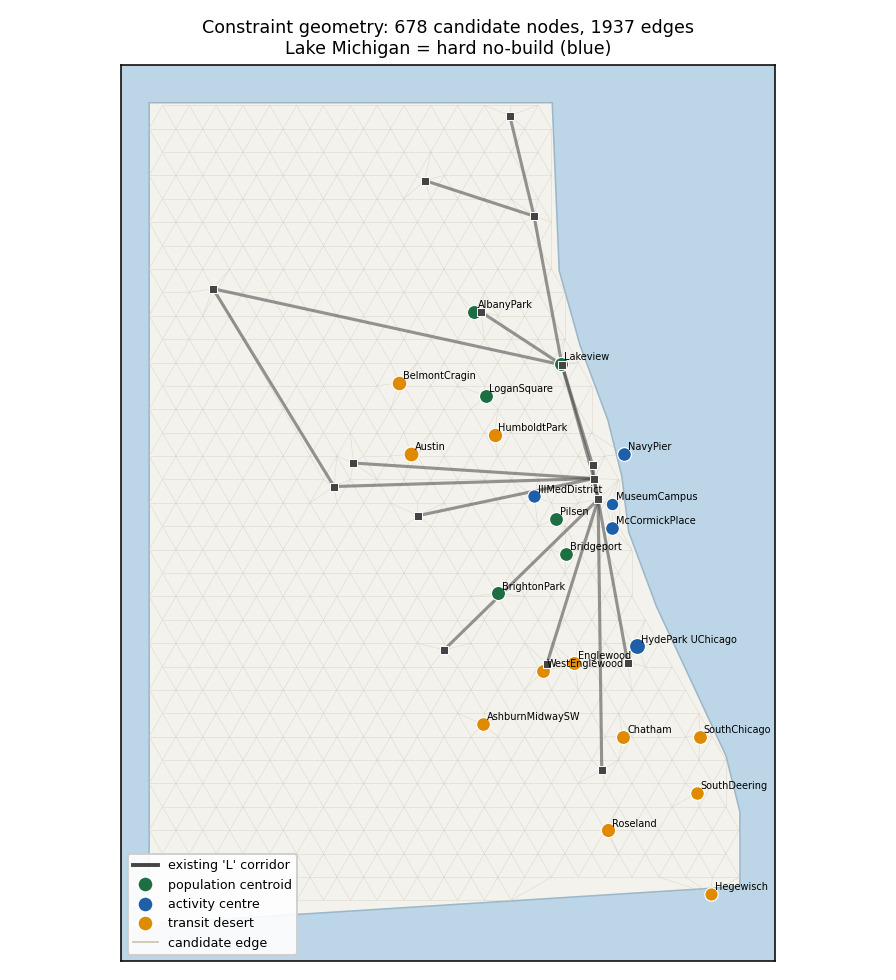
\includegraphics[width=0.62\textwidth]{fig1_candidate_graph.png}
\caption{Constraint geometry. Faint grey: candidate lattice edges. Dark grey:
existing `L' corridors (schematic). Markers: demand nodes colored by dominant role
(green population, blue activity center, orange transit desert), sized by total demand
weight. Blue: Lake Michigan hard no-build boundary.}
\label{fig:cand}
\end{figure}

\subsection{Demand model}
Each demand node $i$ carries three normalized sub-scores in $[0,1]$: residential
population density $\rho_i$, activity-center / employment draw $a_i$, and transit-desert
severity $u_i$ (assembled from community-area populations, major trip generators, and
published Chicago transit-desert maps). Following the user's requested ``weighted mix,''
the demand weight is the convex combination
\begin{equation}
w_i \;=\; \alpha\,\rho_i + \beta\,a_i + \kappa\,u_i, \qquad (\alpha,\beta,\kappa)=(0.4,0.3,0.3).
\label{eq:weight}
\end{equation}
Loading uses the multi-city methodology of \citet{tero2010}: each timestep draws a batch
of source/sink terminal pairs with probability proportional to $w$, and sets the injected
current for a pair $(s,t)$ to $I_0=I_{\text{scale}}\sqrt{w_s w_t}$, so high-demand origin
--destination pairs drive proportionally more flux and reinforce the tubes that serve them.

\subsection{Construction-cost field and effective length}
Real track is not equally expensive everywhere. We define a construction-cost multiplier
$m(\mathbf{x})$ on edge midpoints: $m=0.6$ within $0.7$\,km of an existing corridor
(right-of-way reuse and shared structures lower marginal cost), $m=1.6$ within $2.5$\,km of
the Loop (dense-core tunnelling/elevated premium), and $m=1$ otherwise. The flow physics
sees the \emph{effective} tube length
\begin{equation}
L_{ij} \;=\; \ell_{ij}\, m(\mathbf{x}_{ij}),
\label{eq:Leff}
\end{equation}
where $\ell_{ij}$ is the physical edge length. Because conductance is $\D/L$, costly
corridors present more hydraulic resistance and are selected against, while reported track
kilometers always use the physical $\ell_{ij}$. This is the same device the Tokyo
experiment used --- raising the effective cost of forbidden terrain --- here generalized to
a continuous economic cost surface.

\subsection{Numerical scheme}
We integrate \eqref{eq:adapt} with forward Euler ($dt=0.1$) for $T$ steps, initializing
$\D_{ij}=1+\mathcal{N}(0,0.05)$. Per step we (i) assemble the conductance Laplacian, (ii)
solve \eqref{eq:kirchhoff} simultaneously for a batch of $12$ demand-weighted pairs via a
single multi-right-hand-side factorization, (iii) average $|Q_{ij}|$ across the batch as the
multi-commodity load, and (iv) update $\D$. The headline run uses $T=500$, $\gamma=1.3$,
$I_{\text{scale}}=6$. The continuous field is discretized into a network by retaining tubes
with $\D_{ij}\ge 0.1\,\max\D$, iteratively pruning non-terminal dead-ends, and reconnecting
any stranded demand node by its cheapest candidate path (a guaranteed-feasibility repair).

\section{Baselines and metrics}
On the \emph{identical} candidate graph and terminal set we compute three references that
each optimize a single objective: the \textbf{minimum spanning tree} (metric-closure MST
over terminals --- the cheapest connected network), the \textbf{Steiner tree}
(Mehlhorn 2-approximation, allowing intermediate junctions), and \textbf{hub-and-spoke}
(shortest cost path from every demand node to the Loop --- naive radial planning). We
evaluate every network with the Tero cost--benefit triple:
\begin{itemize}
\item $TL$ --- total physical track length (km), the capital-cost proxy;
\item $MD$ --- mean shortest-path distance between terminal pairs (km), the transport-efficiency
proxy (lower is better);
\item $FT$ --- fault tolerance, the fraction of edges whose removal disconnects \emph{no}
terminal pair. Only bridges separating two terminal-bearing components are critical, so
$FT = 1 - (\#\,\text{critical bridges})/E$. Any tree has $FT=0$.
\end{itemize}

\section{Results}
\subsection{Self-organized growth}
Figure~\ref{fig:evo} shows the conductivity field collapsing from the uniform lattice
(step 0) onto a sparse, reinforced backbone (step 499). High-demand corridors --- the
north lakefront, the Logan Square--Loop axis, and the spine running south toward Englewood,
Chatham, and Roseland --- thicken, while redundant lattice tubes vanish.

\begin{figure}[t]
\centering
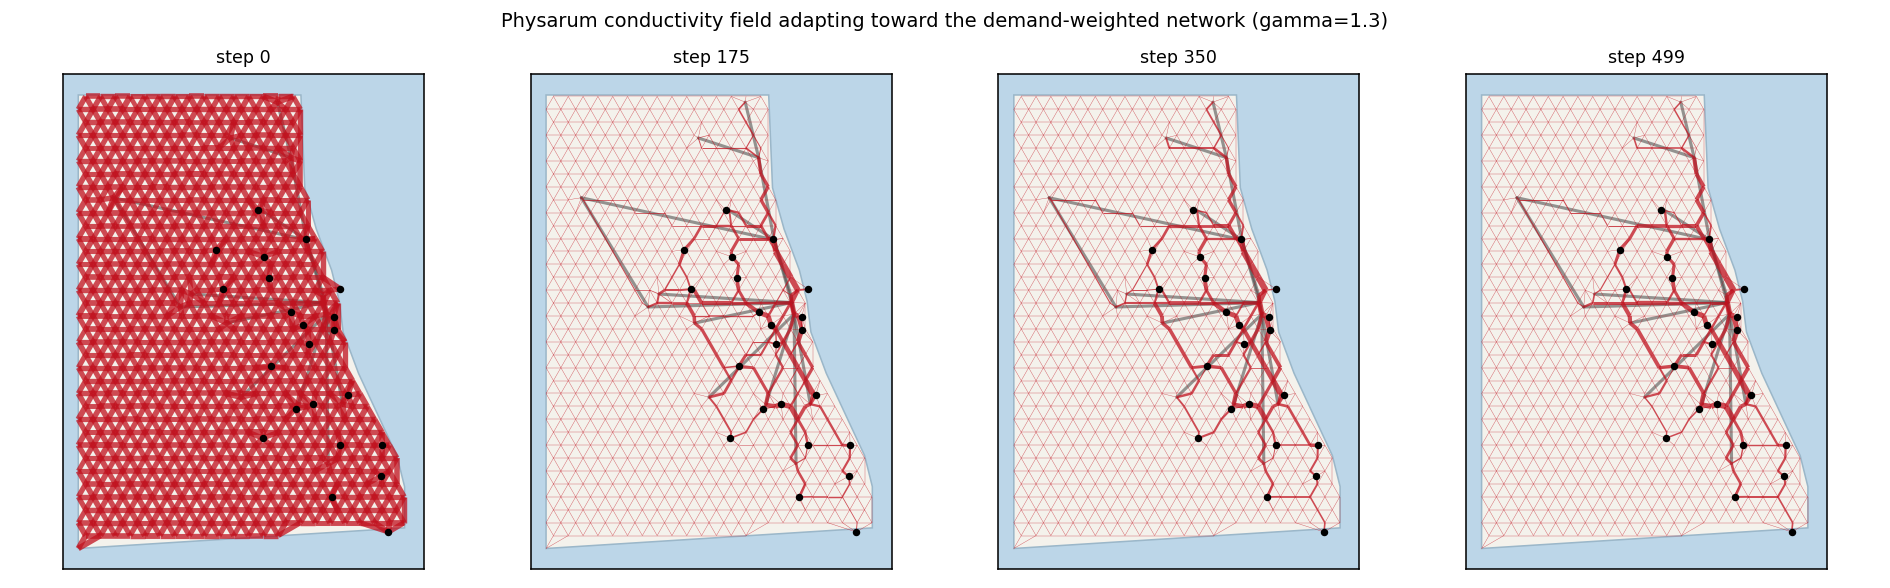
\includegraphics[width=\textwidth]{fig2_evolution.png}
\caption{Adaptation of the tube conductivity field ($\gamma=1.3$). Line width $\propto \D_{ij}$.
The mesh self-prunes toward a demand-weighted backbone.}
\label{fig:evo}
\end{figure}

\subsection{The grown network}
The headline network (Fig.~\ref{fig:grown}) attaches new high-conductivity corridors to the
existing system and reaches every targeted transit desert, including the Far South Side
(Roseland, Hegewisch, South Deering) and the West Side (Austin, Belmont Cragin). It uses
$256$\,km of new track, achieves a mean inter-terminal trip of $18.8$\,km, and a fault
tolerance of $0.89$ --- i.e.\ the overwhelming majority of links can fail without islanding
any demand center, thanks to the loops the model retains.

\begin{figure}[t]
\centering
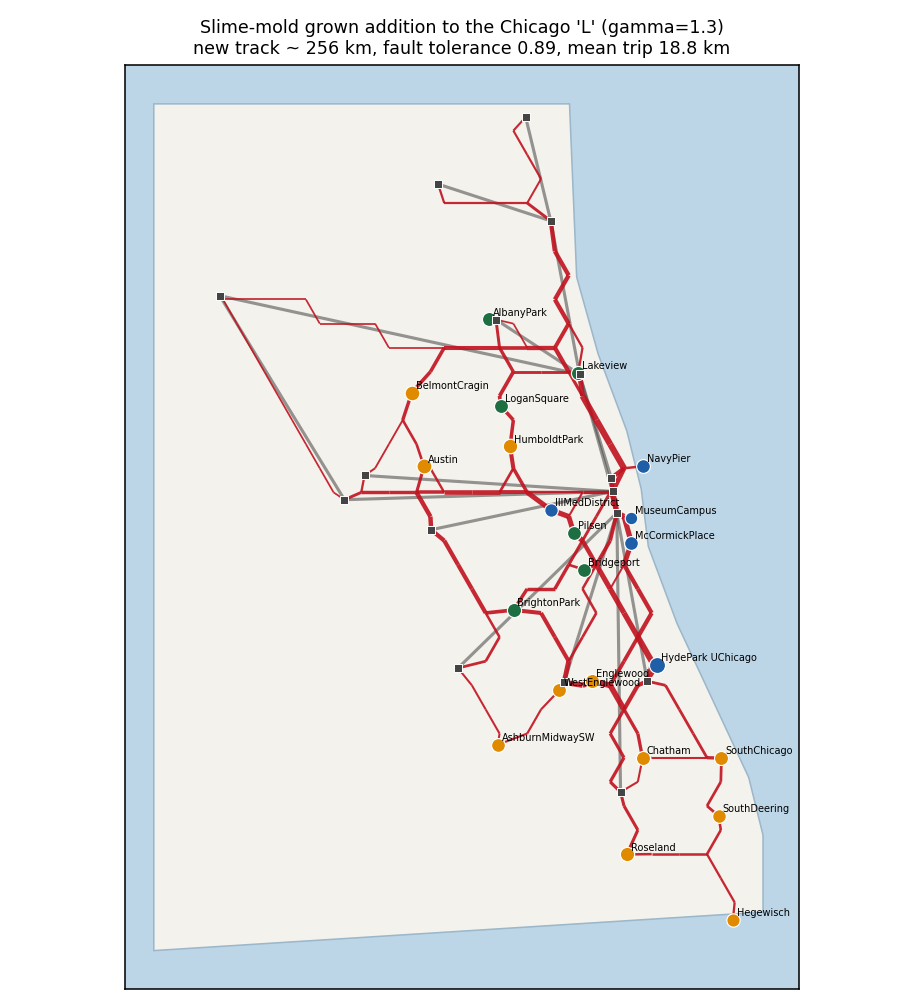
\includegraphics[width=0.66\textwidth]{fig3_grown_network.png}
\caption{Slime-mold grown addition to the Chicago `L' ($\gamma=1.3$). Red tube width
$\propto$ conductivity; grey: existing corridors. The network forms redundant loops on the
dense North/Near-West sides and reaching spurs into the far South and West.}
\label{fig:grown}
\end{figure}

\subsection{Comparison with classical baselines}
Figure~\ref{fig:base} and Table~\ref{tab:metrics} contrast the four designs. The MST and
Steiner trees are cheapest ($\sim$\,$145$\,km) but are \emph{trees}: $FT=0$ and long detoured
trips ($MD\approx 27$--$29$\,km). Hub-and-spoke shortens trips ($MD=19.2$) but remains a
zero-redundancy radial tree. The slime-mold network spends more track to buy what neither
tree can: simultaneous short trips \emph{and} high robustness.

\begin{figure}[t]
\centering
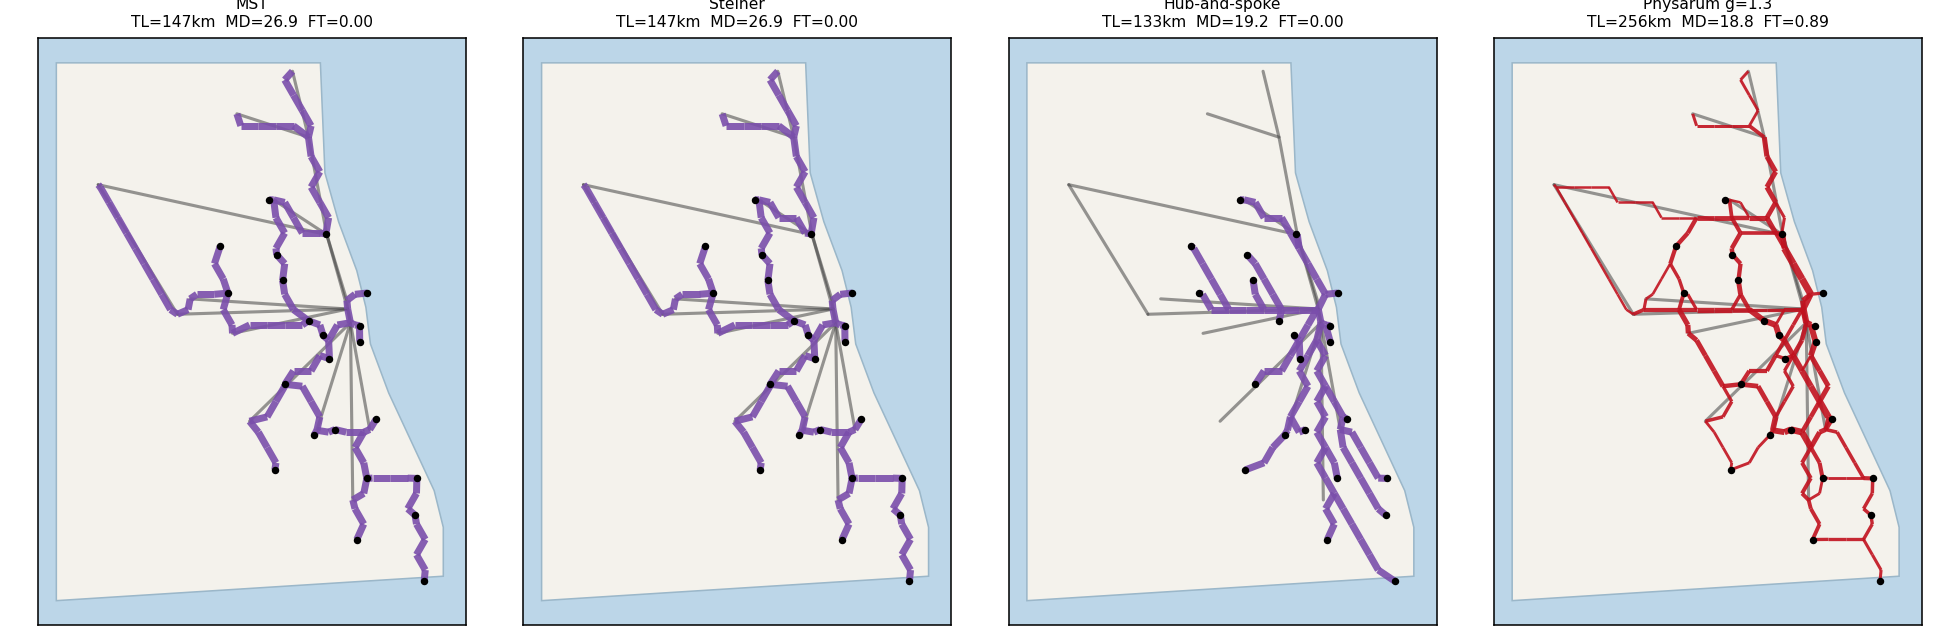
\includegraphics[width=\textwidth]{fig4_baselines.png}
\caption{The four networks on the same candidate graph: MST, Steiner, hub-and-spoke, and the
balanced \emph{Physarum} network.}
\label{fig:base}
\end{figure}

\begin{table}[t]
\centering
\caption{Network metrics on the Chicago candidate graph ($N=678$, $E=1937$, $38$ terminals).
$TL$ total length, $TC$ cost-weighted length, $MD$ mean inter-terminal distance, $FT$ fault
tolerance. Physarum row is the multi-seed mean $\pm$ s.d.\ over 8 seeds.}
\label{tab:metrics}
\begin{tabular}{lrrrrc}
\toprule
Network & $TL$ (km) & $TC$ & $MD$ (km) & $FT$ & connected \\
\midrule
Minimum spanning tree   & $147.0$ & $105.3$ & $26.95$ & $0.00$ & yes \\
Steiner tree (Mehlhorn) & $145.2$ & $111.2$ & $29.29$ & $0.00$ & yes \\
Hub-and-spoke (radial)  & $132.9$ & $\phantom{0}98.9$ & $19.23$ & $0.00$ & yes \\
\textbf{Physarum} $\gamma{=}1.3$ & $247.5\pm11.1$ & $175.7\pm6.4$ & $18.69\pm0.34$ & $0.88\pm0.02$ & yes \\
\bottomrule
\end{tabular}
\end{table}

\subsection{The cost--benefit Pareto front}
Sweeping $\gamma$ traces a continuous frontier (Figs.~\ref{fig:pareto},~\ref{fig:sweep}). As
$\gamma$ falls from $2.2$ to $0.7$ the network grows from a minimal tree ($TL=117$\,km,
$FT=0$) to a dense mesh ($TL=1734$\,km, $FT=1.0$), with fault tolerance and (up to a point)
transport efficiency improving monotonically. Crucially, every \emph{Physarum} point
dominates the trees on the robustness and efficiency axes at a given cost: the baselines sit
on the $FT=0$ floor, whereas $\gamma\in[1.1,1.5]$ delivers $FT=0.76$--$0.95$ for $1.4$--$2.6\times$
the MST length. The ``knee'' near $\gamma=1.3$ is the natural planning choice.

\begin{figure}[t]
\centering
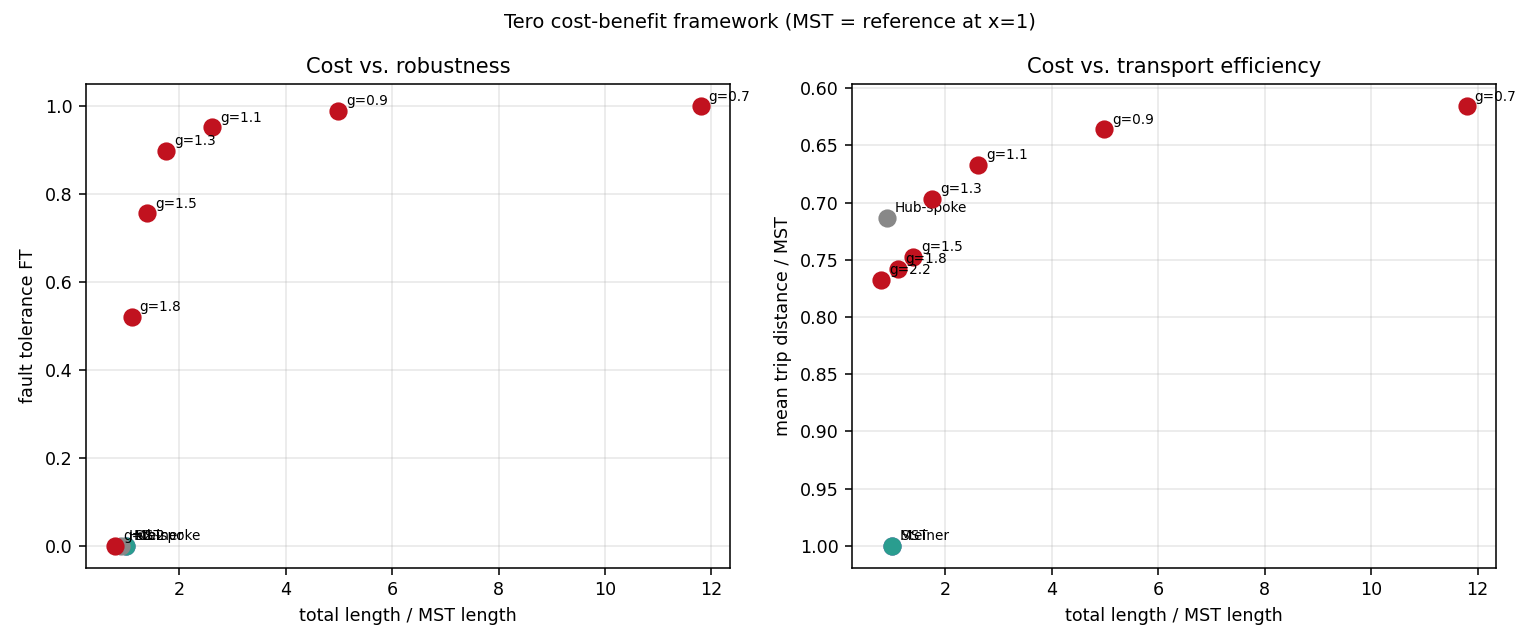
\includegraphics[width=\textwidth]{fig5_pareto.png}
\caption{Tero cost--benefit framework, all networks normalized to the MST. Left: fault
tolerance vs.\ relative length. Right: relative mean trip distance (axis inverted, lower is
better) vs.\ relative length. The \emph{Physarum} family (red) forms a Pareto front the
single-objective baselines cannot reach.}
\label{fig:pareto}
\end{figure}

\begin{figure}[t]
\centering
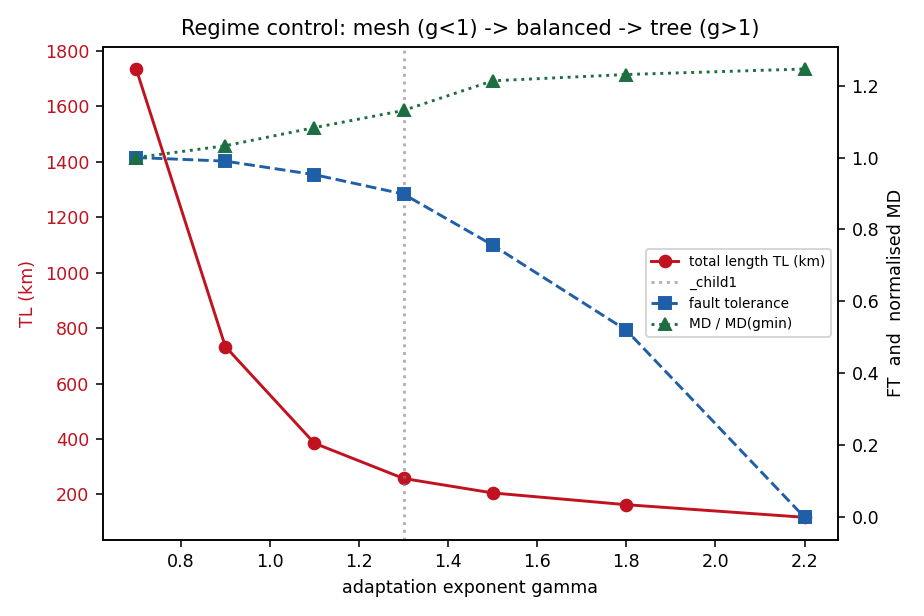
\includegraphics[width=0.62\textwidth]{fig6_gamma_sweep.png}
\caption{Regime control by the adaptation exponent $\gamma$: total length (red, left axis),
fault tolerance and normalized mean distance (right axis). The dotted line marks the headline
$\gamma=1.3$.}
\label{fig:sweep}
\end{figure}

\subsection{Robustness}
Because the loading is stochastic, we repeated the headline run over 8 random seeds. The
metrics are tight --- $TL=247.5\pm11.1$\,km, $MD=18.69\pm0.34$\,km, $FT=0.88\pm0.02$ --- so the
qualitative network (and its quantitative advantage over the trees) is not a seed artifact.

\section{Discussion}
\paragraph{Planning reading.} The model is best understood as a \emph{generative
prior} over network topologies, not a turnkey blueprint. It independently rediscovers
sensible structure: redundant loops where demand is dense (North and Near-West sides) and
single reaching spurs into low-density transit deserts, mirroring how real systems mix
ring/grid cores with radial extensions. The $\gamma$ knob lets a planner dial the
robustness-for-cost exchange explicitly, and the cost field means the network prefers
existing rights-of-way and avoids the expensive core --- both realistic instincts.

\paragraph{Why it beats the trees.} MST and Steiner solve a single objective (minimum cost)
and are therefore maximally fragile. The slime-mold dynamics minimize a \emph{coupled}
dissipation-plus-maintenance functional, which rewards a few load-bearing loops; those loops
are exactly what convert $FT=0$ into $FT\approx 0.9$ and cut detours. The extra length is the
price of robustness, and the Pareto front quantifies that price.

\paragraph{Limitations.} (i) The candidate lattice and schematic existing-line geometry
abstract away street grids, grade, and parcel-level right-of-way; a production model would
ingest GIS centerlines and a true cost raster. (ii) Demand sub-scores are normalized expert
estimates, not a calibrated ridership model; coupling to LODES/ACS origin--destination flows
would sharpen them. (iii) The model captures topology and relative cost, not operations
(headways, transfers, dwell). (iv) Fault tolerance here is a structural (graph) measure, not a
service-level reliability simulation. None of these change the central, seed-stable finding.

\section{Conclusion}
A physics model of slime-mold growth, constrained by Lake Michigan and a construction-cost
surface and loaded by a population/activity/equity demand blend, grows a Chicago `L' expansion
that is markedly more efficient and robust than minimum-spanning-tree, Steiner, or hub-and-spoke
designs at a transparent and tunable length premium. The adaptation exponent $\gamma$ exposes the
entire cost--robustness Pareto front in a single dial, giving planners a principled, reproducible
way to explore expansion topologies before committing to detailed engineering. All code, data,
and figures accompany this document.

\small
\begin{thebibliography}{9}
\bibitem[Bonifaci et al.(2012)]{bonifaci2012} V.~Bonifaci, K.~Mehlhorn, G.~Varma.
Physarum can compute shortest paths. \emph{Journal of Theoretical Biology}, 309:121--133, 2012.
\bibitem[Hwang et al.(1992)]{hwang1992} F.~K.~Hwang, D.~S.~Richards, P.~Winter.
\emph{The Steiner Tree Problem}. North-Holland, 1992.
\bibitem[Nakagaki et al.(2000)]{nakagaki2000} T.~Nakagaki, H.~Yamada, A.~T\'oth.
Maze-solving by an amoeboid organism. \emph{Nature}, 407:470, 2000.
\bibitem[Sun(2017)]{sun2017} Y.~Sun. Physarum-inspired network optimization: A review.
\emph{arXiv:1712.02910}, 2017.
\bibitem[Tero et al.(2007)]{tero2007} A.~Tero, R.~Kobayashi, T.~Nakagaki.
A mathematical model for adaptive transport network in path finding by true slime mold.
\emph{Journal of Theoretical Biology}, 244:553--564, 2007.
\bibitem[Tero et al.(2010)]{tero2010} A.~Tero, S.~Takagi, T.~Saigusa, K.~Ito, D.~P.~Bebber,
M.~D.~Fricker, K.~Yumiki, R.~Kobayashi, T.~Nakagaki. Rules for biologically inspired adaptive
network design. \emph{Science}, 327:439--442, 2010.
\bibitem[Watanabe et al.(2011)]{watanabe2014} S.~Watanabe, A.~Tero, A.~Takamatsu, T.~Nakagaki.
Traffic optimization in railroad networks using an algorithm mimicking an amoeba-like organism.
\emph{Biosystems}, 105:225--232, 2011.
\bibitem[Transit-desert analysis(2025)]{transitdesert2025} Tackling transportation inequality:
Unveiling Chicago's transit deserts and vulnerable communities. \emph{Journal of Urban Planning
and Development}, 151(3), 2025.
\end{thebibliography}

\end{document}
